\section{Abschluss}
Sowohl das Frontend als auch die Smartphone-Apps für Android und iOS sind nun erfolgreich entwickelt und getestet. In
der Abbildung~\ref{fig:umsetzung_zielarchitektur_4} auf Seite~\pageref{fig:umsetzung_zielarchitektur_4} ist die
Gesamtarchitektur mit dem Frontend auf der linken Seite und dem Backend auf der rechten Seite aufgezeigt.

Die Kommunikation der beiden Module erfolgt über den in der Mitte angelegten API Connect Service in der IBM Cloud,
welcher als API-Gateway fungiert und anfallende Anfragen um Informationen erweitert und anschließend weiterleitet.

Die Architektur ist somit erfolgreich umgesetzt und kann von einem Endnutzer genutzt werden, um Vorhersagen für die
aktuellen Bosch Wiegeeinheiten zu erhalten.

Im nächsten Schritt soll die erstellte Architektur nun auf weitere Maschinen angewandt werden. Um dies zu zeigen, wird
im Kapitel~\ref{ch:adaptierbarkeit} ab Seite~\pageref{ch:adaptierbarkeit} die Adaptierbarkeit der Architektur
aufgezeigt.

Damit soll erreicht werden, dass weitere Maschinen in der Produktpalette der Robert Bosch GmbH die Vorteile von
künstlicher Intelligenz im Bereich der Parameteroptimierung erfahren können.

Dafür werden weitere neuronale Netze für die einzelnen Maschinen angelegt und das Frontend dahingehend erweitert,
dass neue Daten eingegeben werden können.

\begin{figure}[h]
    \centering
    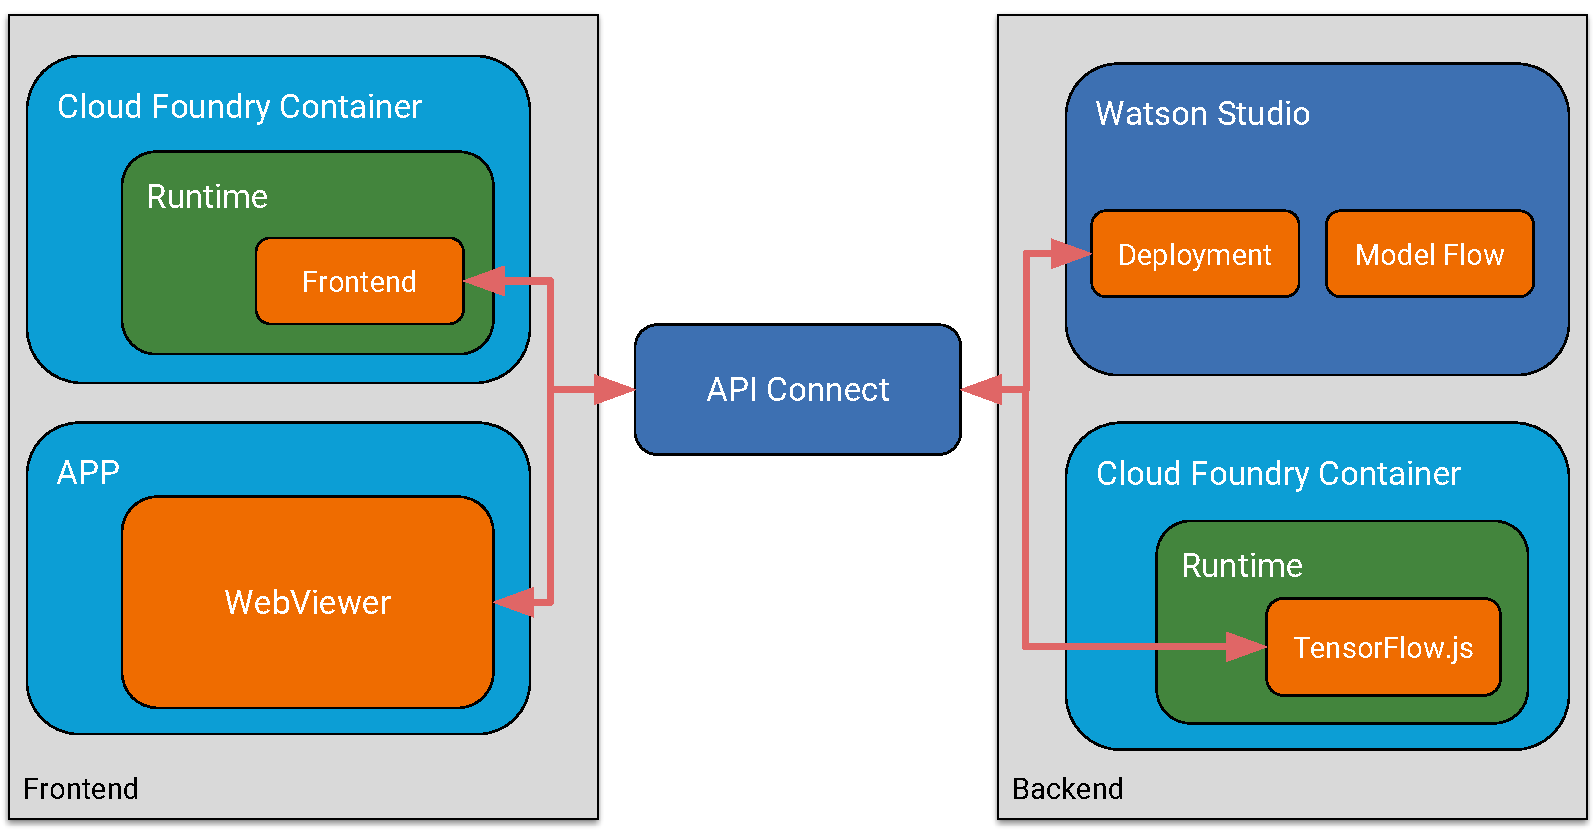
\includegraphics[width=\textwidth]{images/kapitel_4/architektur_uebersicht.pdf}
    \caption{Übersicht der Zielarchitektur}
    \label{fig:umsetzung_zielarchitektur_4}
\end{figure}
